% !TeX TS-program = xelatex
% !BIB TS-program = bibtex

% Full instructions available at:
% https://github.com/pcafrica/focus-beamertheme


\documentclass{beamer}
\usepackage{blindtext} %This package generates automatic text
\usepackage{epigraph}
\usepackage{bussproofs}
\usepackage{amssymb}
\usepackage{listings}

\usepackage{tikz}
\usetikzlibrary{arrows.meta, positioning}
\usetheme{focus}
\usepackage{listings}
\lstset{
  basicstyle=\ttfamily\small,
  frame=single,
  keepspaces=true,
  showstringspaces=false,
  columns=fullflexible,
  escapeinside={(*@}{@*)}  % <- this allows inline math
}
\newcommand{\tvdash}{\mathrel{\text{\textbar\!\textminus}}}

\definecolor{main}{RGB}{142, 111, 62}
% \definecolor{text}{RGB}{60, 60, 80}
% \definecolor{background}{RGB}{255, 255, 255}

\title{An Effect System for Algebraic Effects \& Handlers}
% \subtitle{Subtitle}
\author{Asha}
\titlegraphic{\epigraph{Programming Languages are like saddles, We don't make the saddle for the horse, The horse doesn't need the saddle, It does not want it}{\textit{Andrej Bauer \\ OPLSS 2018}}}

% \titlegraphic{\includegraphics[scale=1.25]{focus-logo.pdf}}
% \institute{Institute Name \\ Institute Address}
\date{\today}

% Footline info is printed only if [numbering=fullbar].
%\footlineinfo{Custom footline text}

\begin{document}
    \input{beginning}
    
    % Use starred version (e.g. \section*{Section name})
    % to disable (sub)section page.
    
    % \input{tt}
    \section{Introductions}
\subsection{Algebraic Effects \& Handlers}


\begin{frame}{The Problem with Traditional Type Systems}
  \begin{itemize}
    \item Traditional type systems describe \textbf{entities of pure computation}, but not \textbf{computational effects}.
    \vspace{0.5em}
    \item Effects (like exceptions, I/O, state) are:
      \begin{itemize}
        \item Invisible to the type system
        \item Difficult to reason about or restrict
        \item Cause code to be less modular and harder to verify
      \end{itemize}
    \vspace{0.5em}
    \item There is a need to unify the formal definition of computational effects under some abstract definition.
  \end{itemize}
\end{frame}
\begin{frame}{What Are Algebraic Effects?}
  \begin{itemize}
    \item \textbf{Algebraic effects} describe computational effects via \textit{abstract operations}.
    \vspace{0.5em}
    \item Examples:
      \begin{itemize}
        \item \texttt{raise : string $\to$ $\_$} \hfill (exceptions)
        \item \texttt{get : unit $\to$ int} \hfill (state)
        \item \texttt{choose : unit $\to$ bool} \hfill (nondeterminism)
      \end{itemize}
    \vspace{0.5em}
    \item Think of them as \textbf{requests} for effects, not implementations.
    \vspace{0.5em}
    \item Separate the notion of \textit{what an effect is} from \textit{how it is handled}.
  \end{itemize}
\end{frame}
% \begin{frame}{What Are Algebraic Effects?}
% \centering
% 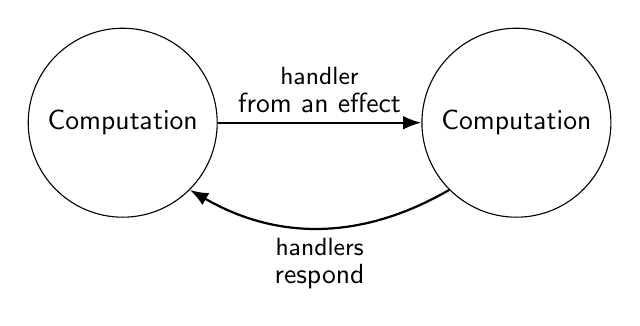
\begin{tikzpicture}[
    every node/.style={font=\sffamily},
    computation/.style={draw, circle, minimum size=2.4cm, align=center},
    >=Latex
]

% Nodes
\node[computation] (C1) at (0, 0) {Computation};
\node[computation] (C2) at (5, 0) {Computation};

% Arrows
\draw[->, thick] (C1.east) -- node[above, align=center] {\small handler\\[-2pt]from an effect} (C2.west);
\draw[<-, thick] (C1.south east) to[bend right=30] node[below, align=center] {\small handlers\\[-2pt]respond} (C2.south west);

\end{tikzpicture}
% \end{frame}

\begin{frame}{Handlers: The Dual Viewpoint}
  \begin{columns}[c]
    \column{0.55\textwidth}
    \begin{itemize}
      \item \textbf{Handlers} define how effects are interpreted.
      \vspace{0.5em}
      \item Think of them as \textbf{responders} to abstract operations.
      \vspace{0.5em}
      \item Example clauses:
      \begin{itemize}
        \item \texttt{val x $\Rightarrow$ c\textsubscript{val}}
        \item \texttt{op y k $\Rightarrow$ c\textsubscript{op}}
      \end{itemize}
      \vspace{0.5em}
      \item First-class and composable.
    \end{itemize}

    \column{0.45\textwidth}
    \centering
    % \includegraphics[width=0.9\textwidth]{computation_handler_diagram.png}
    \resizebox{0.8\linewidth}{!}{%
  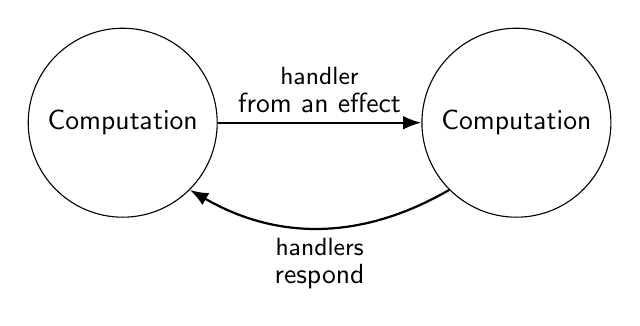
\begin{tikzpicture}[
    every node/.style={font=\sffamily},
    computation/.style={draw, circle, minimum size=2.4cm, align=center},
    >=Latex
]

% Nodes
\node[computation] (C1) at (0, 0) {Computation};
\node[computation] (C2) at (5, 0) {Computation};

% Arrows
\draw[->, thick] (C1.east) -- node[above, align=center] {\small handler\\[-2pt]from an effect} (C2.west);
\draw[<-, thick] (C1.south east) to[bend right=30] node[below, align=center] {\small handlers\\[-2pt]respond} (C2.south west);

\end{tikzpicture}
}
    
  \end{columns}
\end{frame}

\begin{frame}[fragile]{Motivation Through Examples}
\vspace{-0.5em}
\begin{block}{Nondeterministic Choice with \texttt{Choose}}
\begin{verbatim}
effect Choose : unit -> bool

let flip = Choose()

with handler
  val x => x
  | Choose() k => k(true) || k(false)
handle
  if flip then "Heads" else "Tails"
\end{verbatim}
\end{block}
\vspace{0.5em}
\begin{itemize}
  \item \texttt{Choose()} is an effect request — “flip a coin”
  \item Handler responds by exploring \texttt{true} and \texttt{false}
  \item Result: evaluates to both “Heads” and “Tails”
\end{itemize}
\end{frame}

\begin{frame}[fragile]{Message Passing: \texttt{Send} and \texttt{Receive} Effects}
\vspace{-0.5em}
\begin{block}{\scriptsize Effect Declarations and \texttt{ping}}
\begin{scriptsize}
\begin{verbatim}
effect Send : int -> unit
effect Receive : unit -> int

let ping =
  for i = 1 to 3 do
    Send(i);
    let msg = Receive() in
    Printf.printf "Ping received %d\n" msg
  done
\end{verbatim}
\end{scriptsize}
\end{block}
\vspace{0.3em}
\begin{itemize}
  \item \texttt{Send} and \texttt{Receive} are abstract operations.
  \item \texttt{ping} sends values and receives replies.
  \item Handler decides what message passing means.
\end{itemize}
\end{frame}
\begin{frame}[fragile]{Message Passing: The \texttt{pong} Side}
\vspace{-0.5em}
\begin{block}{\scriptsize \texttt{pong} Responds to \texttt{ping}}
\begin{scriptsize}
\begin{verbatim}
let pong =
  for _ = 1 to 3 do
    let msg = Receive() in
    Printf.printf "Pong received %d\n" msg;
    Send(msg + 100)
  done
\end{verbatim}
\end{scriptsize}
\end{block}
\vspace{0.3em}
\begin{itemize}
  \item \texttt{pong} waits for a message, processes it, and replies.
  \item Sends back \texttt{msg + 100} after each receive.
  \item This effectful back-and-forth models structured concurrency.
\end{itemize}
\end{frame}

\begin{frame}[fragile]{Message Passing via Effects: Part 3}
\vspace{-0.5em}
\begin{block}{\scriptsize The \texttt{run} Function Coordinates Both}
\begin{scriptsize}
\begin{verbatim}
let rec run pingside pongside =
  match pingside () with
  | v -> v
  | effect (Send x) k1 ->
    match pongside () with
    | v -> v
    | effect Receive k2 ->
      run (fun () -> continue k1 ()) (fun () -> continue k2 x)
  | _ -> failwith "Unexpected effect"
\end{verbatim}
\end{scriptsize}
\end{block}

\begin{itemize}
  \item Handles \texttt{Send} from \texttt{ping}, \texttt{Receive} from \texttt{pong}.
  \item Resumes each with continuation-passed values.
  \item Models **cooperative message passing** purely via effects.
\end{itemize}
\end{frame}
\begin{frame}[fragile]{6a: Programs Stay Pure, Effects Are Handled}
\vspace{-0.5em}
\begin{block}{\scriptsize Define Effects and Suspension State}
\begin{scriptsize}
\begin{verbatim}
effect Send : int -> unit
effect Receive : unit -> int

type state =
  | Done
  | Paused of int * continuation
  | PausedR of continuation
\end{verbatim}
\end{scriptsize}
\end{block}

\begin{itemize}
  \item Programs use effects via \texttt{perform}.
  \item They don’t define what sending/receiving means.
  \item Interpretation is delegated to the handler.
\end{itemize}
\end{frame}
\begin{frame}[fragile]{6b: Programs as Pure Computations}
\vspace{-0.5em}
\begin{block}{\scriptsize Handlers Manage Interaction, Not the Programs}
\begin{scriptsize}
\begin{verbatim}
let rec ping n =
  if n > 0 then (
    let m = perform (Send n);
    Printf.printf "ping sent %d\n" m;
    ping (n - 1)
    
  else 
    return ()
  )

let rec pong () =
  let n = perform Receive in
  Printf.printf "pong received %d\n" n;
  pong ()
\end{verbatim}
\end{scriptsize}
\end{block}

\begin{itemize}
  \item \texttt{ping} and \texttt{pong} describe logic only.
  \item They don’t care who receives or replies.
  \item They are \textbf{pure} computations.
\end{itemize}
\end{frame}
\begin{frame}[fragile]{6c: Handlers for \texttt{ping} and \texttt{pong}}
\vspace{-0.5em}
\begin{block}{\scriptsize Handlers Pause and Resume Computations}
\begin{scriptsize}
\begin{verbatim}
handler e 
| unit |-> Done
| Send x |-> 
    fun k -> Paused (x, k)
| Receive () |->
    fun k -> PausedR k
        
\end{verbatim}
\end{scriptsize}
\end{block}

\begin{itemize}
  \item Each handler manages its own computation.
  \item Sending pauses the program; receiving continues it.
\end{itemize}
\end{frame}
\begin{frame}[fragile]{6d: Driving Interaction with \texttt{run\_both}}
\vspace{-0.5em}
\begin{block}{\scriptsize Resuming Ping and Pong Step by Step}
\begin{scriptsize}
\begin{verbatim}
let rec run_both p po =
  match p with
  | Done -> ()
  | Paused x k ->
    match po with
    | PausedR k' -> run_both (k ()) (k' x)
\end{verbatim}
\end{scriptsize}
\end{block}

\begin{itemize}
  \item \texttt{run\_both} drives both computations cooperatively.
  \item At each step, \texttt{ping} sends, then \texttt{pong} receives and responds.
  \item Effect handling is decoupled from computation structure.
\end{itemize}
\end{frame}

\begin{frame}{The Goal of the Paper}
\begin{itemize}
  \item Propose an \textbf{effect system} for a core language with algebraic effects and handlers.
  \item Track \textbf{computational effects} directly in types.
  \item Provide a formal \textbf{operational semantics} and \textbf{type system}.
  \item Handle practical challenges:
  \begin{itemize}
    \item \textbf{Poisoning problem}: how unhandled effects can spread.
    \item \textbf{Subtyping} of effects and polymorphism.
    \item \textbf{Coherence}: different derivations of typing should agree.
  \end{itemize}
  \item Keep the system small and expressive: \textbf{Core Eff}.
\end{itemize}
\end{frame}
    \section{Syntax of Core Eff}
\begin{frame}{Core Eff Syntax: Values}
\textbf{Values (\texttt{v}):}
\begin{itemize}
  \item \texttt{x} \hfill (variable)
  \item \texttt{fun x $\Rightarrow$ c} \hfill (function abstraction)
  \item \texttt{handler val x $\Rightarrow$ c\textsubscript{v} \\
  \hspace{3.5em} | op x k $\Rightarrow$ c\textsubscript{op}} \hfill (handler)
\end{itemize}

\vspace{1em}
Values are inert — they do not trigger computation by themselves.  
Handlers are first-class values that define what to do with operations.
\end{frame}
\begin{frame}{Core Eff Syntax: Computations}
\textbf{Computations (\texttt{c}):}
\begin{itemize}
  \item \texttt{val v} \hfill (pure return)
  \item \texttt{v v'} \hfill (function application)
  \item \texttt{let x = c$_1$ in c$_2$} \hfill (sequential binding)
  \item \texttt{e \# op v} \hfill (invoke operation \texttt{op} on effect instance \texttt{e})
  \item \texttt{with v handle c} \hfill (handle computation with \texttt{v})
\end{itemize}

\vspace{1em}
Computations represent steps of execution.  
They may perform effects and must be run to produce results.
\end{frame}


\begin{frame}{Core Eff Syntax: Types (with \texttt{E$^R$})}
\textbf{Pure types (\texttt{A, B}):}
\begin{itemize}
  \item \texttt{bool} \hfill (booleans)
  \item \texttt{nat} \hfill (natural numbers)
  \item \texttt{E$^R$} \hfill (effect instance: name of effect \texttt{E} at region \texttt{R})
  \item \texttt{A $\rightarrow$ C} \hfill (functions from pure to computation)
  \item \texttt{C $\Rightarrow$ D} \hfill (handlers from computation to computation)
\end{itemize}

\vspace{1em}
\textbf{Dirty types (\texttt{C}):}
\begin{itemize}
  \item \texttt{A ! $\Delta$} \hfill (computations returning \texttt{A} and performing effects $\Delta$)
\end{itemize}

\vspace{1em}
\textbf{Explanation:}
\begin{itemize}
  \item \texttt{E$^R$} is the type of an \textbf{effect instance}.
  \item \texttt{E} is an effect (like \texttt{State} or \texttt{IO}), \texttt{R} is a \textbf{region variable} that scopes the instance.
  \item Effect instances are passed as pure values and used in operations (e.g., \texttt{e \# op v}).
\end{itemize}
\end{frame}

\begin{frame}{Regions, Dirt, and Operation Signatures}

\textbf{Region variables (\( R \)):}
\begin{itemize}
  \item Abstract names that identify \textbf{effect instances}.
  \item Appear in types like \( E^R \), where \( E \) is an effect (e.g., State, Exception).
  \item Allow fine-grained tracking of effects tied to specific instances.
\end{itemize}

\vspace{1em}
\textbf{Dirt (\( \Delta \)):}
\begin{itemize}
  \item A \textbf{finite set of operations} the computation may perform.
  \item Each element has the form \( \iota \# \texttt{op} \), where \( \iota \) is an effect instance.
  \item Appears in dirty types: \( A ! \Delta \)
\end{itemize}

\vspace{1em}
\textbf{Effect signature (\( \Sigma \)):}
\begin{itemize}
  \item Maps each effect name \( E \) to a set of operations:
  \[
    \Sigma(E) = \{ \texttt{op}_i : A_i \rightarrow B_i \}
  \]
  \item Each operation has a parameter type \( A_i \) and result type \( B_i \).
\end{itemize}

\end{frame}

\begin{frame}{Core Eff: Effect Sets and Interpretation}
\textbf{Effect set $\Delta$:}
\begin{itemize}
  \item A finite set of operations the computation may perform.
  \item Written as \texttt{\{State.get, Exn.raise, IO.print\}}, etc.
\end{itemize}

\vspace{1em}
\textbf{Effectful computation type:}
\begin{itemize}
  \item \texttt{int ! \{State.get, State.put\}} \\
    means the computation returns an \texttt{int}, but may access state.
\end{itemize}

\vspace{1em}
\textbf{Key idea:} types describe both \textit{what is computed} and \textit{what effects may occur}.
\end{frame}

\begin{frame}{Pure vs Dirty Types}
\textbf{Pure types:}
\begin{itemize}
  \item Describe \textbf{values only}.
  \item Examples:
    \begin{itemize}
      \item \texttt{nat}, \texttt{bool}, \texttt{E$^R$}
      \item \texttt{nat $\rightarrow$ bool ! $\Delta$} (functions)
      \item \texttt{C $\Rightarrow$ D} (handlers)
    \end{itemize}
  \item Cannot perform any effect on their own.
\end{itemize}

\vspace{1em}
\textbf{Dirty types:}
\begin{itemize}
  \item Describe \textbf{computations}.
  \item Syntax: \texttt{A ! $\Delta$}
  \item Means: produces a value of type \texttt{A} and may perform effects in $\Delta$.
  \item Example: \texttt{bool ! \{State.get, State.put\}}
\end{itemize}

\vspace{1em}
\textbf{Key distinction:} only dirty types describe computations that can perform effects.
\end{frame}

\begin{frame}{Function and Handler Types in Action}
\textbf{Function types:} \texttt{A $\rightarrow$ C}
\begin{itemize}
  \item Takes a \textbf{pure argument} of type \texttt{A}
  \item Returns a \textbf{dirty computation} of type \texttt{C}
  \item Example: \texttt{nat $\rightarrow$ bool ! \{Exn.raise\}}
\end{itemize}

\vspace{1em}
\textbf{Handler types:} \texttt{C $\Rightarrow$ D}
\begin{itemize}
  \item Transforms a computation of type \texttt{C} into one of type \texttt{D}
  \item Typically used with \texttt{with h handle c}
  \item Example:
    \begin{itemize}
      \item \texttt{bool ! \{Choose\} $\Rightarrow$ list bool ! \{\}} \\
        (handler that explores both choices and returns all outcomes)
    \end{itemize}
\end{itemize}

\vspace{1em}
\textbf{Note:} Handlers are values that accept and transform computations.
\end{frame}

\begin{frame}{Overview of Typing Rules}
\begin{itemize}
  \item The typing system tracks both:
  \begin{itemize}
    \item \textbf{Pure types} (e.g., \texttt{bool}, \texttt{nat}): values with no effects.
    \item \textbf{Dirty types} (e.g., \texttt{bool ! \{Exn.raise\}}): computations that may perform effects.
  \end{itemize}

  \item \textbf{Effect annotations} describe which operations a computation may perform.
  \begin{itemize}
    \item Example: \texttt{A ! \{State.get, Exn.raise\}}
  \end{itemize}

  \item \textbf{Typing rules} ensure:
  \begin{itemize}
    \item Effectful programs are properly annotated.
    \item Handlers transform computations safely.
    \item Subtyping works with effect sets.
  \end{itemize}

  \item \textbf{Key challenge:} Combining effects and continuations while preserving type safety.
\end{itemize}
\end{frame}
    \section{Operational Semantics Of Core-Eff}

\begin{frame}{Operational Semantics: Values and \texttt{val}}
\textbf{Values:}
\[
v ::= x \mid \texttt{fun } x \Rightarrow c \mid \texttt{handler } \cdots
\]
\begin{itemize}
  \item Values are fully evaluated and are not reducible.
\end{itemize}

\vspace{1em}
\textbf{Computation form:}
\[
\texttt{val } v
\]
\begin{itemize}
  \item A computation that simply returns value \( v \).
  \item This is a \emph{terminal configuration} under the small-step semantics.
  \item There is \textbf{no reduction rule} for \texttt{val v}, i.e., no \( \texttt{val } v \rightsquigarrow \cdots \)
\end{itemize}

\vspace{1em}
This is the base case for computations — the final result before effects or handlers are involved.
\end{frame}

\begin{frame}{Small-Step Semantics: \texttt{if} and \texttt{match}}

\textbf{Conditional branching:}
\[
\frac{}{\texttt{if true then } c_1 \texttt{ else } c_2 \rightsquigarrow c_1}
\]
\[
\frac{}{\texttt{if false then } c_1 \texttt{ else } c_2 \rightsquigarrow c_2}
\]

\vspace{1em}
\textbf{Pattern matching:}
\[
\frac{}{\texttt{match } 0 \texttt{ with } 0 \Rightarrow c_1 \mid S\,x \Rightarrow c_2 \mapsto c_1}
\]
\[
\frac{}{\texttt{match } S\,v \texttt{ with } 0 \Rightarrow c_1 \mid S\,x \Rightarrow c_2 \mapsto c_2[v/x]}
\]

\vspace{1em}
\textbf{Note:} \texttt{if} and \texttt{match} reduce only when their scrutinees are values.
\end{frame}

\begin{frame}{Small-Step Semantics: \texttt{fun}, \texttt{let}, and \texttt{with}}

\textbf{Function application:}
\[
\frac{}{(\texttt{fun } x \Rightarrow c)\ v \rightsquigarrow c[v/x]}
\]

\vspace{1em}
\textbf{Let-binding:}
\[
\frac{}{ \texttt{let } x = \texttt{val } v \texttt{ in } c \rightsquigarrow c[v/x] }
\]
\[
\frac{c_1 \rightsquigarrow c_1'}{\texttt{let } x = c_1 \texttt{ in } c_2 \rightsquigarrow \texttt{let } x = c_1' \texttt{ in } c_2}
\]

\vspace{1em}
\textbf{Handler congruence:}
\[
\frac{c \rightsquigarrow c'}{\texttt{with } e \texttt{ handle } c \rightsquigarrow \texttt{with } e \texttt{ handle } c'}
\]

% \vspace{1em}
% Only one subterm is reduced per step — all rules are in left-to-right evaluation order.
\end{frame}

\begin{frame}{Small-Step Semantics: Effect Invocation}
\textbf{Effect operation call:}
\[
\frac{}{
  \texttt{let } x = \iota \# \texttt{op } e \texttt{ in } c
  \rightsquigarrow
  \iota \# \texttt{op } e (y.\ \texttt{let } x = y \texttt{ in } c)
}
\]

\vspace{1.5em}
\textbf{Explanation:}
\pause
\begin{itemize}
  \item This rule models an \emph{unhandled effect}. So for the effect to be handled the operation must be propogated with this rule.
  \item It suspends the computation, exposing the continuation as a function of the result.
  \item The handler, if present, will later match and resume from this.
\end{itemize}
\end{frame}

% \begin{frame}{Small-Step Semantics: Handling Operations (Full Rule)}

% \textbf{Handler (operation case):}
% \[
% \frac{
%   \begin{array}{l}
%     h = \texttt{handler val } x \Rightarrow c_v \mid \texttt{op } x\ k \Rightarrow c_{op} \\
%     r = \iota \# \texttt{op } e\ (y.c) \\
%     \\
%     \texttt{with } h\ \texttt{handle } r \rightsquigarrow c_{op}
%     [e/x,\ (\texttt{fun } y \Rightarrow \texttt{with } h\ \texttt{handle } c)/k]
%   \end{array}
% }{
%   \texttt{with } h\ \texttt{handle } r \rightsquigarrow \cdots
% }
% \]

% \vspace{1em}
% This rule applies when an operation \texttt{op} from instance \(\iota\) is matched by handler \(h\),
% and constructs a resumption to continue the suspended computation.
% \end{frame}
\begin{frame}{Small-Step Semantics: Handler Rule }

\[
\frac{
  h = \texttt{handler val } x \mapsto c_v \mid ocs
  \qquad
  (op: A^{op} \rightarrow B^{op}) \in \Sigma_E
}{
\begin{aligned}
  & \texttt{with } h \texttt{ handle } (\iota \# \texttt{op } e\ (y.c)) \rightsquigarrow \\
  & ocs_{ \iota \# \texttt{op }} (e, \lambda y:B^{op} \mapsto \texttt{with } h \texttt{ handle } c)
\end{aligned}
}
\]

% \begin{prooftree}
%     \AxiomC{$$h = \texttt{handler val } x \mapsto c_v \mid ocs$$}
%     \AxiomC{$$(op: A^{op} \rightarrow B^{op}) \in \Sigma_E$$}
%     \BinaryInfC{
%     $$
%     \begin{aligned}
%   & \texttt{with } h \texttt{ handle } (\iota \# \texttt{op } e\ (y.c)) \rightsquigarrow \\
%   & ocs_{ \iota \# \texttt{op }} (e, \lambda y:B^{op} \mapsto \texttt{with } h \texttt{ handle } c)

% \end{aligned}
% $$
% }
% \end{prooftree}

where

\begin{aligned}
& (nil)_{\iota \# \texttt{op }}(e,\kappa) = \iota \# \texttt{op } e (y. \kappa y) \hfill \\
& (\iota' \# \texttt{op' } x k \mapsto c \mid ocs)_{\iota \# \texttt{op }} (e, \kappa) =
\begin{cases}
      c [ e/x, \kappa / k ] & \text{if }\ \iota \# \texttt{op} = \iota' \# \texttt{op' } \\
      ocs_{\iota \# \texttt{op}}(e, \kappa) & \text{otherwise}
    \end{cases}
\end{aligned}

\end{frame}

\begin{frame}{Example: Handling an Operation — \texttt{Choose}}

\textbf{Effect:}
\[
\texttt{effect Choose : unit} \rightarrow \texttt{bool}
\]

\textbf{Computation:}
\[
\texttt{let x = perform (Choose ()) in if x then 1 else 2}
\]

\textbf{Handler:}
\[
\texttt{handler val x} \mapsto [x] \mid
\texttt{Choose } u\ k \mapsto k(\texttt{true}) @ k(\texttt{false})
\]

% \vspace{1em}
\textbf{Operational Step:}
\[
\texttt{with h handle let x = } \iota \# \texttt{Choose () in if x then 1 else 2} 
\rightsquigarrow \\
\texttt{let x = true in if x then 1 else 2} @
\texttt{let x = false in if x then 1 else 2}
\]

% \vspace{1em}
% \textbf{Handler applies the rule:}
% \begin{itemize}
%   \item Matches operation: \( \iota \# \texttt{Choose} \)
%   \item Binds \( e = () \)
%   \item Continuation \( \kappa = \lambda y.\ \texttt{with h handle let x = y in if x then 1 else 2} \)
%   \item Resumes with both \( \texttt{true} \) and \( \texttt{false} \)
% \end{itemize}
\end{frame}

% \begin{frame}{Example 3.1 — Initial Term Under Handler}

% \[
% \\
% \texttt{with } h \texttt{ handle }\\
% \texttt{let } x_1 = \iota \# \texttt{lookup }() \texttt{ in } \\
% \texttt{let } x_2 = \iota \# \texttt{update } x_1 \texttt{ in }
% \texttt{val (succ } x_1)
% \]

% \vspace{1em}
% \textbf{Handler:}
% \[
% \texttt{handler}
% \begin{cases}
% \texttt{val } x \mapsto \iota \# \texttt{update } x \\
% \iota \# \texttt{lookup } x\ k \mapsto k\ 1 \\
% \iota \# \texttt{update } x\ k \mapsto k\ ()
% \end{cases}
% \]

% \vspace{1em}
% \textbf{Goal:} Reduce this computation step-by-step according to the Core Eff small-step semantics.
% \end{frame}

\begin{frame}{Example 3.1 — Initial Configuration}

\textbf{Expression:}
\begin{align*}
&\texttt{with } h\ \texttt{handle let } x_1 = \iota \# \texttt{lookup }() \\
&\quad \texttt{in let } x_2 = \iota \# \texttt{update } x_1 \\
&\quad \texttt{in val (succ } x_1)
\end{align*}

\textbf{Handler:}
\[
\texttt{handler}
\begin{cases}
  \texttt{val } x \mapsto \iota \# \texttt{update } x \\
  \iota \# \texttt{lookup } x\ k \mapsto k\ 1 \\
  \iota \# \texttt{update } x\ k \mapsto k\ ()
\end{cases}
\]
\end{frame}

\begin{frame}{Step 1 — Suspend \texttt{lookup}}

\begin{align*}
&\texttt{let } x_1 = \iota \# \texttt{lookup }() \texttt{ in } c \\
&\rightsquigarrow \iota \# \texttt{lookup }() \left(y_1.\ \texttt{let } x_1 = \texttt{val } y_1 \texttt{ in } c\right)
\end{align*}

Apply to our term:
\begin{align*}
&\texttt{with } h\ \texttt{handle } \iota \# \texttt{lookup }() \Big(y_1. \texttt{let } x_1 = \texttt{val } y_1 \\
&\quad \texttt{in let } x_2 = \iota \# \texttt{update } x_1 \\
&\quad \texttt{in val (succ } x_1)\Big)
\end{align*}
\end{frame}

\begin{frame}{Step 2 — Apply \texttt{lookup} Handler}

Handler clause:
\[
\iota \# \texttt{lookup } x\ k \mapsto k\ 1
\]

Apply:
\begin{align*}
k &= \lambda y_1.\ \texttt{with } h\ \texttt{handle let } x_1 = \texttt{val } y_1 \\
  &\quad \texttt{in let } x_2 = \iota \# \texttt{update } x_1 \\
  &\quad \texttt{in val (succ } x_1)
\end{align*}

\textbf{Substitute 1 for \( y_1 \):}
\begin{align*}
&\texttt{with } h\ \texttt{handle let } x_1 = \texttt{val } 1 \\
&\quad \texttt{in let } x_2 = \iota \# \texttt{update } x_1 \\
&\quad \texttt{in val (succ } x_1)
\end{align*}
\end{frame}


\begin{frame}{Step 3 — Reduce \texttt{update} and \texttt{succ}}

\textbf{Substitute \( x_1 = 1 \):}
\begin{align*}
&\texttt{with } h\ \texttt{handle let } x_2 = \iota \# \texttt{update } 1 \texttt{ in val } 2
\end{align*}

\textbf{Desugar generic effect:}
\begin{align*}
&\equiv \texttt{with } h\ \texttt{handle let } x_2 = \iota \# \texttt{update } 1\ (y_2.\ \texttt{val } y_2) \\
&\quad \texttt{in val } 2
\end{align*}
\end{frame}

 \begin{frame}{Step 4 — Handle Second Operation}

Suspend:
\begin{align*}
&\rightsquigarrow \texttt{with } h\ \texttt{handle } \iota \# \texttt{update } 1 \\
&\quad \left(y_2.\ \texttt{let } x_2 = \texttt{val } y_2 \texttt{ in val } 2\right)
\end{align*}

Handler clause:
\[
\iota \# \texttt{update } x\ k \mapsto k\ ()
\]

Apply:
\begin{align*}
&\rightsquigarrow \texttt{with } h\ \texttt{handle let } x_2 = \texttt{val } () \texttt{ in val } 2 \\
&\rightsquigarrow \texttt{with } h\ \texttt{handle val } 2
\end{align*}
\end{frame}

\begin{frame}{Step 5 — Final Handler Clause Applies}

Handler clause:
\[
\texttt{val } x \mapsto \iota \# \texttt{update } x
\]

Apply:
\[
\texttt{with } h\ \texttt{handle val } 2
\rightsquigarrow
\iota \# \texttt{update } 2
\]

\vspace{1em}
\textbf{Final result:}
\[
\iota \# \texttt{update } 2
\]

This update is not handled — it escapes the scope of the handler.
\end{frame}

\begin{frame}{Big-Step Semantics: Core Judgment}

\textbf{Form of the judgment:}
\[
\langle c, h \rangle \Downarrow r
\]

\textbf{Meaning:}
\begin{itemize}
  \item Under handler \( h \), computation \( c \) evaluates to result \( r \).
  \item This result is either:
    \begin{itemize}
      \item A value: \( \texttt{val } v \)
      \item A suspended operation: \( \iota \# \texttt{op } e (y.c) \)
    \end{itemize}
  \item The handler may handle effects as evaluation proceeds.
\end{itemize}
\end{frame}

\begin{frame}{Big-Step Semantics: Possible Results}

\textbf{Results \( r \) have two forms:}
\[
r ::= \texttt{val } v \quad \mid \quad \iota \# \texttt{op } e (y.c)
\]

\textbf{Interpretation:}
\begin{itemize}
  \item \( \texttt{val } v \): the computation completed with value \( v \)
  \item \( \iota \# \texttt{op } e (y.c) \):
    \begin{itemize}
      \item An operation \( \texttt{op} \) was performed on instance \( \iota \)
      \item \( e \) is the argument
      \item \( y.c \) is the continuation (what happens next)
    \end{itemize}
\end{itemize}
\end{frame}

\begin{frame}{Big-Step Semantics: Rule Format}

Each rule is of the form:
\[
\frac{\text{premises}}{\langle c, h \rangle \Downarrow r}
\]

\textbf{Example:}
\[
\frac{}{\langle \texttt{val } v, h \rangle \Downarrow \texttt{val } v}
\]

This is the base case — returning a value directly.
\end{frame}

% \begin{frame}{Big-Step Semantics: Evaluation Judgment}

% \textbf{Judgment:}
% \[
% c \Downarrow r
% \]

% \textbf{Result \(r\):}
% \[
% r ::= \texttt{val } e \quad \mid \quad \iota \# \texttt{op } e (x. c)
% \]

% \vspace{1em}
% \textbf{Interpretation:}
% \begin{itemize}
%   \item \(c\) evaluates to a value \(e\), or
%   \item suspends on an operation \(\iota \# \texttt{op}\), with continuation \(x.c\)
% \end{itemize}
% \end{frame}

% \begin{frame}{Big-Step Semantics: Base Cases}

% \begin{align*}
% &\frac{}{\texttt{val } e \Downarrow \texttt{val } e} \\
% &\frac{}{\iota \# \texttt{op } e (x. c) \Downarrow \iota \# \texttt{op } e (x. c)}
% \end{align*}

% \vspace{1em}
% \textbf{A value returns itself, and an operation suspends immediately.}
% \end{frame}

\begin{frame}{Big-Step Semantics: Evaluation Judgment}

\textbf{Judgment:}
\[
c \Downarrow r
\]

\textbf{Result \(r\):}
\[
r ::= \texttt{val } e \quad \mid \quad \iota \# \texttt{op } e (x. c)
\]

\vspace{1em}
\textbf{Interpretation:}
\begin{itemize}
  \item \(c\) evaluates to a value \(e\), or
  \item suspends on an operation \(\iota \# \texttt{op}\), with continuation \(x.c\)
\end{itemize}
\end{frame}

\begin{frame}{Big-Step Semantics: Base Cases}

\begin{align*}
&\frac{}{\texttt{val } e \Downarrow \texttt{val } e} \\
&\frac{}{\iota \# \texttt{op } e (x. c) \Downarrow \iota \# \texttt{op } e (x. c)}
\end{align*}

\vspace{1em}
\textbf{A value returns itself, and an operation suspends immediately.}
\end{frame}

\begin{frame}{Big-Step Semantics: Let Binding}

\begin{align*}
&\frac{c_1 \Downarrow \texttt{val } e \quad c_2[e/x] \Downarrow r}
{\texttt{let } x = c_1 \texttt{ in } c_2 \Downarrow r}
\\[1em]
&\frac{c_1 \Downarrow \iota \# \texttt{op } e (y. c)}
{\texttt{let } x = c_1 \texttt{ in } c_2 \Downarrow \iota \# \texttt{op } e (y. \texttt{let } x = c \texttt{ in } c_2)}
\end{align*}
\end{frame}

\begin{frame}{Big-Step Semantics: Conditionals and Matches}

\begin{align*}
&\frac{c_1 \Downarrow r}
{\texttt{if true then } c_1 \texttt{ else } c_2 \Downarrow r}
\\
&\frac{c_2 \Downarrow r}
{\texttt{if false then } c_1 \texttt{ else } c_2 \Downarrow r}
\\[1em]
&\frac{c_1 \Downarrow r}
{\texttt{match } 0 \texttt{ with } 0 \mapsto c_1 \mid \texttt{succ } x \mapsto c_2 \Downarrow r}
\\
&\frac{c_2[e/x] \Downarrow r}
{\texttt{match succ } e \texttt{ with } 0 \mapsto c_1 \mid \texttt{succ } x \mapsto c_2 \Downarrow r}
\end{align*}
\end{frame}

\begin{frame}{Big-Step Semantics: Application and Recursion}

\begin{align*}
&\frac{c[e/x] \Downarrow r}
{(\texttt{fun } x \mapsto c)\ e \Downarrow r}
\\[1em]
&\frac{c_2[(\texttt{fun } x \mapsto \texttt{let rec } f x = c_1 \texttt{ in } c_1)/f] \Downarrow r}
{\texttt{let rec } f x = c_1 \texttt{ in } c_2 \Downarrow r}
\end{align*}
\end{frame}
\begin{frame}{Handler Semantics: Handling \texttt{val}}

\textbf{Handler:}
\[
h = \texttt{handler val } x \mapsto c_v \mid \texttt{op } x\ k \mapsto c_{\text{op}}
\]

\textbf{Rule:}
\[
\frac{c \Downarrow \texttt{val } e \quad c_v[e/x] \Downarrow r}
{\texttt{with } h \texttt{ handle } c \Downarrow r}
\]

\vspace{1em}
\textbf{Interpretation:}
\begin{itemize}
  \item If computation \( c \) evaluates to a value,
  \item we substitute into the handler's \texttt{val} clause and evaluate it.
\end{itemize}
\end{frame}
\begin{frame}{Handler Semantics: Handling an Operation}

\textbf{Handler:}
\[
h = \texttt{handler val } x \mapsto c_v \mid \texttt{op } x\ k \mapsto c_{\text{op}}
\]

\textbf{Rule:}
\[
\frac{
  c \Downarrow \iota \# \texttt{op } e (y. c') \quad
  c_{\text{op}}[e/x,\ \lambda y.\ \texttt{with } h \texttt{ handle } c'/k] \Downarrow r
}{
  \texttt{with } h \texttt{ handle } c \Downarrow r
}
\]

\vspace{1em}
\textbf{Interpretation:}
\begin{itemize}
  \item If \( c \) suspends on an operation matched by \( h \),
  \item we apply the handler’s \texttt{op} clause,
  \item passing the argument \( e \) and a resumable continuation.
\end{itemize}
\end{frame}

\begin{frame}{Handler Semantics: Forwarding Unhandled Operations}

\textbf{Rule (when operation is not handled):}
\[
\frac{
  c \Downarrow \iota \# \texttt{op } e (y. c') \quad
  r = \iota \# \texttt{op } e (y.\ \texttt{with } h \texttt{ handle } c')
}{
  \texttt{with } h \texttt{ handle } c \Downarrow r
}
\]

\vspace{1em}
\textbf{Interpretation:}
\begin{itemize}
  \item If the handler does not match the operation,
  \item we re-emit it, wrapping the continuation with the same handler.
\end{itemize}
\end{frame}

\begin{frame}{Proposition 3.2 — Semantic Equivalence}

\textbf{Statement:}
\[
c \rightsquigarrow^{*} r \quad \Longleftrightarrow \quad c \Downarrow r
\]

\vspace{1em}
\textbf{Explanation:}
\begin{itemize}
  \item \( \rightsquigarrow^{*} \): zero or more steps of the small-step reduction.
  \item \( \Downarrow \): big-step evaluation to result \( r \).
  \item \( r \): either a value \( \texttt{val } v \) or a suspended operation \( \iota \# \texttt{op } e (x. c) \).
\end{itemize}

\vspace{1em}
\textbf{Interpretation:}
\begin{itemize}
  \item Big-step and small-step semantics produce the same results.
  \item This ensures both operational models are equivalent and interchangeable.
\end{itemize}

\end{frame}
    \section{An Effect System}
\subsection{Intro and Poisoning}

\begin{frame}{Section 4: An Effect System}

\textbf{Goal:}
\begin{itemize}
  \item Extend the type system to track not just \emph{what} a program computes,
  but also \emph{which operations} it may perform.
  \item Types become \textbf{dirty} — they carry information about effects.
\end{itemize}

\vspace{1em}
\textbf{Motivation:}
\begin{itemize}
  \item Distinguish between pure and effectful computations.
  \item Enable more modular reasoning about side effects.
  \item Support features like effect polymorphism and effect masking.
\end{itemize}

\end{frame}

\begin{frame}{The Poisoning Problem: Motivation}

\textbf{Issue:} A function that \emph{could be pure} may be marked as effectful due to how it is defined.

\vspace{1em}
\textbf{Cause:}
\begin{itemize}
  \item In Core Eff, functions are first-class and effectful computations are values.
  \item This means we can return functions from effectful contexts.
  \item However, if such a function is returned from within a computation that performs effects, the \emph{entire function} may be marked as dirty — even if it doesn’t perform any effects.
\end{itemize}

\vspace{1em}
\textbf{Consequence:}
\begin{itemize}
  \item The function type becomes \emph{poisoned} by unrelated effects.
  \item Makes type signatures overly conservative and imprecise.
\end{itemize}

\end{frame}

\begin{frame}{The Poisoning Problem:  Example}

\textbf{Assume:}
\begin{itemize}
  \item A ground type \texttt{string}
  \item An effect instance \( \texttt{std} : \texttt{Console}^R \), with:
    \[
    \Sigma(\texttt{Console}) = \{ \texttt{write} : \texttt{string} \rightarrow \texttt{unit} \}
    \]
\end{itemize}

\vspace{1em}
\textbf{Consider:}
\begin{align*}
& \texttt{let ignore} = \texttt{val (fun msg} \mapsto \texttt{val ()}) \\
& \texttt{let f} = \texttt{if } b \texttt{ then (val ignore)} \\ 
& \texttt{else val (std\#write) in val ignore}
\end{align*}

\vspace{1em}
\textbf{What is the type of \texttt{ignore}?}
\begin{itemize}
  \item Ideally: \quad \( \texttt{string} \rightarrow \texttt{unit} \;!\; \emptyset \)
  \item But in the conditional: \( \texttt{string} \rightarrow \texttt{unit} \;!\; \{ \texttt{std}\#\texttt{write} \} \)
\end{itemize}
\textbf{Problem:} the \texttt{ignore} function is pure, but gets \textbf{over-typed} due to context.
\end{frame}

\begin{frame}{Solving Poisoning via Subtyping}

\textbf{Key idea:}
\begin{itemize}
  \item Allow a dirty type \( A\ !\ \Delta \) to be treated as \( A\ !\ \Delta' \) when \( \Delta' \subseteq \Delta \).
  \item This lets us safely discard “irrelevant” effects from a type when they are not used.
\end{itemize}

\vspace{1em}
\textbf{In the example:}
\[
\texttt{string} \rightarrow \texttt{unit} \;!\; \{ \texttt{std}\#\texttt{write} \}
\le
\texttt{string} \rightarrow \texttt{unit} \;!\; \emptyset
\]

\vspace{1em}
\textbf{Benefit:}
\begin{itemize}
  \item Avoids over-tainting pure expressions.
  \item Makes the type system more precise and modular.
\end{itemize}
\end{frame}

\begin{frame}{Dirty Type Subtyping Rule}

\textbf{Subtyping on dirty types:}
\[
\frac{A = A' \quad \Delta' \subseteq \Delta}
{A\ !\ \Delta \leq A'\ !\ \Delta'}
\]

\vspace{1em}
\textbf{This rule allows:}
\begin{itemize}
  \item Weakening the dirt component of a type
  \item No change in the result type \( A \)
\end{itemize}

\vspace{1em}
\textbf{Notation:} \( A\ !\ \Delta \leq A\ !\ \Delta' \)  
means: we can treat a computation that may perform \( \Delta \) as one that may perform any smaller set \( \Delta' \)
\end{frame}

\begin{frame}{Core Eff Syntax: Types (with Dirt)}

\textbf{Value types} \( A, B \) and \textbf{Computation types} \( C \) are defined as:

\begin{align*}
A, B ::= &\quad \alpha \quad \text{(type variable)} \\
        &\mid \texttt{bool} \mid \texttt{nat} \mid \texttt{string} \mid \dots \\
        &\mid A \rightarrow C \quad \text{(function type)} \\
        &\mid E^R \quad \text{(effect instance of type } E \text{ at region } R) \\
        &\mid \texttt{handler } C \Rightarrow D \quad \text{(handler type)}
\end{align*}

\vspace{0.5em}

\begin{align*}
C, D ::= A\ !\ \Delta \quad \text{(computation type with dirt)}
\end{align*}

\vspace{1em}

\textbf{Dirt} \( \Delta \): a finite set of operation labels of the form \( \iota \# \texttt{op} \)

\end{frame}

\begin{frame}{Effect Signatures, Regions, and Dirt}

\textbf{Effect Signature \( \Sigma \):}
\[
\Sigma(E) = \{ \texttt{op}_i : A_i \rightarrow B_i \}_{i \in I}
\quad \text{for each effect name } E
\]

\vspace{0.5em}
\textbf{Effect Instances:}
\[
\iota : E^R
\quad \text{means } \iota \text{ is an instance of effect } E \text{ in region } R
\]

\vspace{1em}
\textbf{Operation Labels:}
\[
\iota \# \texttt{op}
\quad \text{identifies the operation } \texttt{op} \text{ performed on instance } \iota
\]

\vspace{1em}
\textbf{Dirt:}
\[
\Delta \subseteq \{ \iota \# \texttt{op} \}
\quad \text{is a finite set of operation labels}
\]

\vspace{1em}
\textbf{Dirty type:}
\[
A\ !\ \Delta \quad \text{means: computation returning } A \text{ may perform effects } \Delta
\]

\end{frame}
\subsection{Type system}
\begin{frame}{Typing Judgments and Contexts}

\textbf{Typing judgments:}
$$
\Gamma \tvdash e : A
\qquad
\Gamma \tvdash c : A\ !\ \Delta
$$

\begin{itemize}
  \item \( e \): a pure expression, producing a value of type \( A \)
  \item \( c \): a computation, producing a result of type \( A \), possibly performing effects \( \Delta \)
\end{itemize}

\vspace{1em}
\textbf{Typing context \( \Gamma \):}
\begin{itemize}
  \item A finite set of assumptions of the form:
    \begin{itemize}
      \item \( x : A \) — term variables
      \item \( \alpha \) — type variables
      \item \( R \) — region variables
    \end{itemize}
\end{itemize}

\vspace{1em}
\textbf{Note:} We write \( \Gamma, x : A \tvdash e : B \) to extend contexts.
\end{frame}

\begin{frame}{Typing Rules: Constants and Variables}

\textbf{Pure value judgments:}
\[
\Gamma \tvdash e : A
\]

\vspace{1em}

\[
\frac{c : \texttt{const of type } A}
{\Gamma \tvdash c : A}
\quad\textsc{(Const)}
\]

\vspace{1em}

\[
\frac{x : A \in \Gamma}
{\Gamma \tvdash x : A}
\quad\textsc{(Var)}
\]

\end{frame}

\begin{frame}{Typing Rules: Functions and Applications}

\textbf{Judgment form:}
\[
\Gamma \tvdash e : A
\qquad
\Gamma \tvdash c : A\ !\ \Delta
\]

\vspace{1em}

\textbf{Function abstraction:}
\[
\frac{\Gamma, x : A \tvdash c : B\ !\ \Delta}
{\Gamma \tvdash \texttt{fun } x \mapsto c : A \rightarrow B\ !\ \Delta}
\quad\textsc{(Fun)}
\]

\vspace{1.5em}

\textbf{Function application:}
\[
\frac{
  \Gamma \tvdash v_1 : A \rightarrow B\ !\ \Delta
  \quad
  \Gamma \tvdash v_2 : A
}{
  \Gamma \tvdash v_1\ v_2 : B\ !\ \Delta
}
\quad\textsc{(App)}
\]

\end{frame}

\begin{frame}{Typing Rule: \texttt{val} (Subtyping-Safe)}

\textbf{Rule:}
\[
\frac{\Gamma \tvdash e : A}
{\Gamma \tvdash \texttt{val } e : A\ !\ \emptyset}
\quad\textsc{(Val)}
\]

\vspace{1em}
\textbf{Key Point:}
\begin{itemize}
  \item The `val` construct lifts a pure expression into a pure computation.
  \item The resulting computation has dirt \( \emptyset \).
\end{itemize}

\vspace{1em}
\textbf{Why this is general:}
\begin{itemize}
  \item Due to subtyping:
  \[
  A\ !\ \emptyset \leq A\ !\ \Delta \quad \text{for any } \Delta
  \]
  \item This allows us to type `val e` at any dirt level needed downstream.
\end{itemize}

\end{frame}

\begin{frame}{Typing Rule: \texttt{let}}

\textbf{Rule:}
\[
\frac{
  \Gamma \tvdash c_1 : A\ !\ \Delta_1
  \quad
  \Gamma, x : A \tvdash c_2 : B\ !\ \Delta_2
}{
  \Gamma \tvdash \texttt{let } x = c_1 \texttt{ in } c_2 : B\ !\ \Delta_1 \cup \Delta_2
}
\quad\textsc{(Let)}
\]

\vspace{1em}
\textbf{Interpretation:}
\begin{itemize}
  \item Run \( c_1 \), bind its result to \( x \), then run \( c_2 \).
  \item All effects from both computations are accumulated.
\end{itemize}

\end{frame}

\begin{frame}{Typing Rule: Sequencing \texttt{c₁ ; c₂}}

\textbf{Rule:}
\[
\frac{
  \Gamma \tvdash c_1 : A\ !\ \Delta_1
  \quad
  \Gamma \tvdash c_2 : B\ !\ \Delta_2
}{
  \Gamma \tvdash c_1\ ;\ c_2 : B\ !\ \Delta_1 \cup \Delta_2
}
\quad\textsc{(Seq)}
\]

\vspace{1em}
\textbf{Interpretation:}
\begin{itemize}
  \item Run \( c_1 \), discard its result, then run \( c_2 \).
  \item The resulting dirt includes effects from both computations.
\end{itemize}

\end{frame}

\begin{frame}{Typing Rule: Operation Call }

\textbf{Assume:}
\begin{itemize}
  \item \( \iota : E^R \in \Gamma \)
  \item \( \texttt{op} : A^{\texttt{op}} \rightarrow B^{\texttt{op}} \in \Sigma(E) \)
\end{itemize}

\vspace{1em}

\textbf{Rule:}
\[
\frac{
  \Gamma, y: B^{op}  \tvdash c : A^{\texttt{op}} \ !\ \Delta
}{
  \Gamma\tvdash \iota \# \texttt{op } c : B^{\texttt{op}} \ !\ \Delta \cup \{ \iota \# \texttt{op} \}
}
\quad\textsc{(Op)}
\]

\vspace{1em}

\textbf{Interpretation:}
\begin{itemize}
  \item The argument \( c \) is itself a computation, not just a pure expression.
  \item The dirt includes the dirt of \( c \), plus the label for the operation call.
  \item This allows for effects to be embedded in the argument to the operation.
\end{itemize}

\end{frame}

\begin{frame}{Typing Rule: Handler Application}

\textbf{Handler typing:}
\[
\Gamma \tvdash h : A\ !\ \Delta \Rightarrow B\ !\ \Delta'
\qquad
\Gamma \tvdash c : A\ !\ \Delta
\]

\textbf{Rule:}
\[
\frac{
  \Gamma \tvdash h : A\ !\ \Delta \Rightarrow B\ !\ \Delta'
  \quad
  \Gamma \tvdash c : A\ !\ \Delta
}{
  \Gamma \tvdash \texttt{with } h \texttt{ handle } c : B\ !\ \Delta'
}
\quad\textsc{(Handle)}
\]

\vspace{1em}

\textbf{Interpretation:}
\begin{itemize}
  \item Handler \( h \) handles all operations in \( \Delta \) performed by \( c \)
  \item Produces a computation of type \( B\ !\ \Delta' \)
  \item The dirt \( \Delta' \) reflects any effects left unhandled by \( h \)
\end{itemize}

\end{frame}

\begin{frame}{Handler Clause Type: \( C / \Delta \)}

\textbf{Notation:}
\[
C / \Delta
\quad \text{means: computation of type } C \text{ with handled dirt } \Delta
\]

\vspace{1em}

\textbf{Example:}
\[
A\ !\ \Delta \;/\; \Delta
\quad \text{means: computation of type } A\ !\ \Delta \text{ with all effects handled}
\]

\vspace{1em}

\textbf{Usage:}
\begin{itemize}
  \item Appears in the type of a handler:
  \[
  \Gamma \tvdash h : A\ !\ \Delta \Rightarrow B\ !\ \Delta'
  \]
  \item The \texttt{val}-clause and each \texttt{op}-clause must be typed against \( C / \Delta \)
  \item It expresses that all operations in \( \Delta \) are handled — and others must not appear
\end{itemize}

\end{frame}

\begin{frame}{Typing Rule: Handler Definition (\textsc{Hand})}

\textbf{Handler has the form:}
\[
\texttt{handler val } x \mapsto c_v \mid \texttt{op}_i\ x\ k \mapsto c_i
\]

\textbf{Rule:}
\[
\frac{
  \Gamma, x : A \tvdash c_v : B\ !\ \Delta'
  \quad
  \Gamma \tvdash \texttt{ocs} : B\ !\ \Delta' / \Delta'' 
  \quad \Delta \subset \Delta' \cup \Delta''
}{
  \Gamma \tvdash h : A\ !\ \Delta \Rightarrow B\ !\ \Delta'
}
\quad\textsc{(Hand)}
\]

\vspace{1em}

\textbf{Interpretation:}
\begin{itemize}
  \item The \texttt{val}-clause transforms results of type \( A \) into computations of type \( B\ !\ \Delta' \)
  \item The op-cases collectively handle all operations in \( \Delta \)
  \item The resulting handler maps \( A\ !\ \Delta \) to \( B\ !\ \Delta' \)
\end{itemize}

\end{frame}

\begin{frame}{Typing Rule: Op-Cases (Empty) — \textsc{OpCases-Nil}}

\textbf{Rule:}
\[
\frac{}{\Gamma \tvdash nil_{C} : A\ !\ C / \emptyset  }
\quad\textsc{(OpCases-Nil)}
\]

\vspace{1em}

\textbf{Interpretation:}
\begin{itemize}
  \item An empty handler (no op-cases) can handle a computation with no effects
  \item This is the base case for building op-cases recursively
  \item The result dirt \( \Delta' \) can still be non-empty — it's from the `val` clause
\end{itemize}

\end{frame}

\begin{frame}{Typing Rule: Op-Cases (Extend) — \textsc{OpCases-Cons}}

\textbf{Exact rule from the paper:}

\[
\frac{
  \begin{array}{l}
    \iota : E^R \in \Gamma \quad\quad \texttt{op} : A^{\texttt{op}} \rightarrow B^{\texttt{op}} \in \Sigma(E) \\
    \Gamma, x : A^{\texttt{op}},\ k : B^{\texttt{op}} \rightarrow C\ !\ \Delta''
    \tvdash c : C\ !\ \Delta'' \\
    \Gamma \tvdash \texttt{ocs} : C\ !\ \Delta''  / \Delta' 
    \quad
    \Delta \subset \Delta' \cup^. R \#op
  \end{array}
}{
  \Gamma \tvdash (\iota \# \texttt{op } x\ k \mapsto c) \mid \texttt{ocs}
  : C !\ \Delta'' / \Delta 
}
\quad\textsc{(OpCases-Cons)}
\]

\end{frame}
    
    \input{end.tex}
   
\end{document}
